\chapter{Validação}

Para validação dos algoritmos foram gerados alguns grafos hipotéticos com cenários distintos.
Muitos deles utilizaram o mesmo vetor de custo, como dito na seção \ref{sec:pathdyn}, que representam
o tempo médio das passagens dos veículos por uma aresta ao longo do dia, em intervalos de 10 minutos.

% \subsection{Cenários de teste}

\section{Ferramenta de simulação do caminho mínimo}
Para determinar o caminho mínimo entre dois pontos conhecidos em grafos dinâmicos, foi criado
uma extensão ao Dynagraph, que simula o caminho mínimo. Para isso, segue a sequência:
\begin{itemize}
\item Ler a estrutura de dados JSON;
\item Exibir o grafo com todos os vértices e arestas;
\item Selecionar um dos 3 algoritmos para cálculo e exibição do caminho mínimo;
\item Baixar o arquivo JSON ou ir para a aplicação Dynagraph, que contém os mesmos dados do grafo mais as arestas do caminho mínimo;
\item Selecionar o dynagraph e abrir o arquivo baixado ();
\end{itemize}

As figuras \ref{fig:shortestpath}, \ref{fig:upperlimit} e \ref{fig:downlimit} mostram captura de telas
da ferramenta exibindo exemplos de caminho mínimo dos 3 algoritmos e os seus dados:

\begin{figure}[htbp]
\centering
 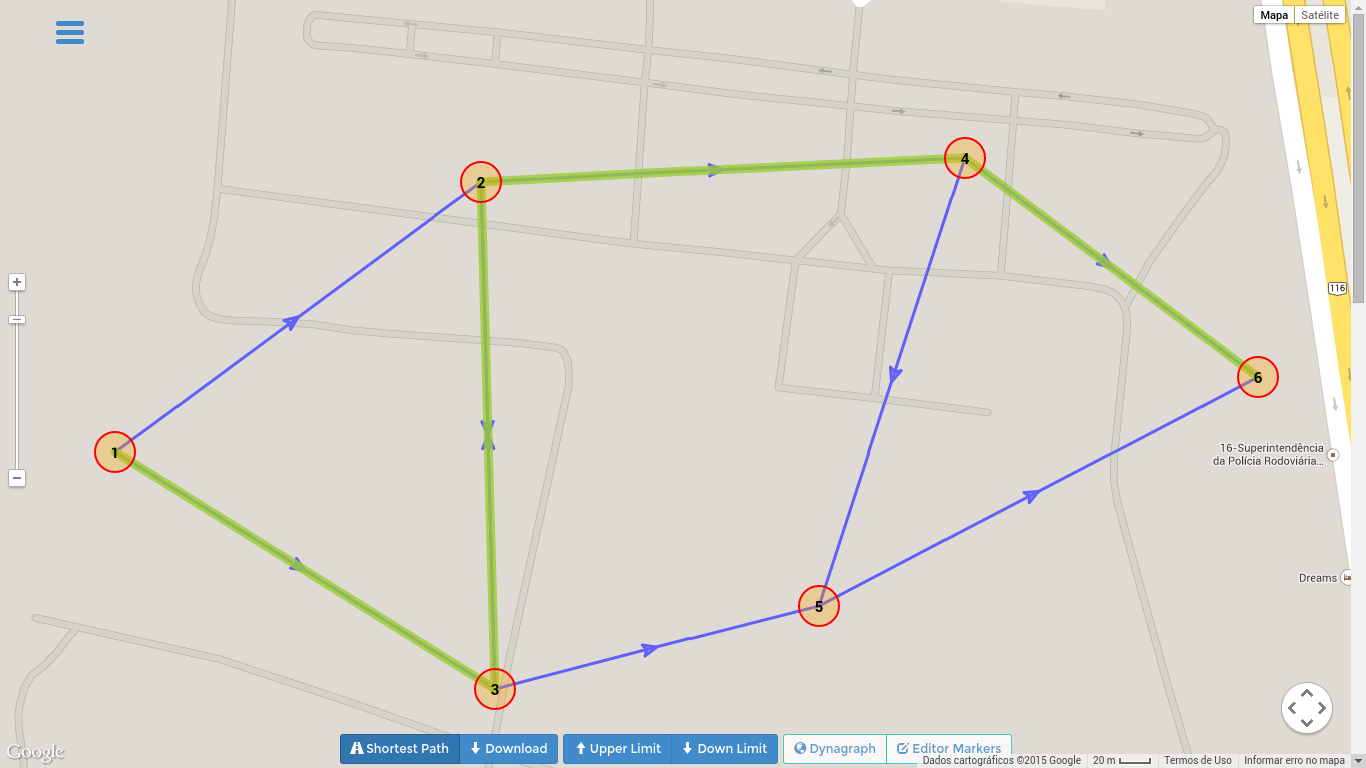
\includegraphics[width=.90\textwidth]{chapters/fig/shortestpath.png}
\caption{Simulador de Caminho Mínimo - Topologia Dinâmica e Atributos Dinâmicos}
\label{fig:shortestpath}
\end{figure}
\FloatBarrier

\begin{figure}[htbp]
\centering
 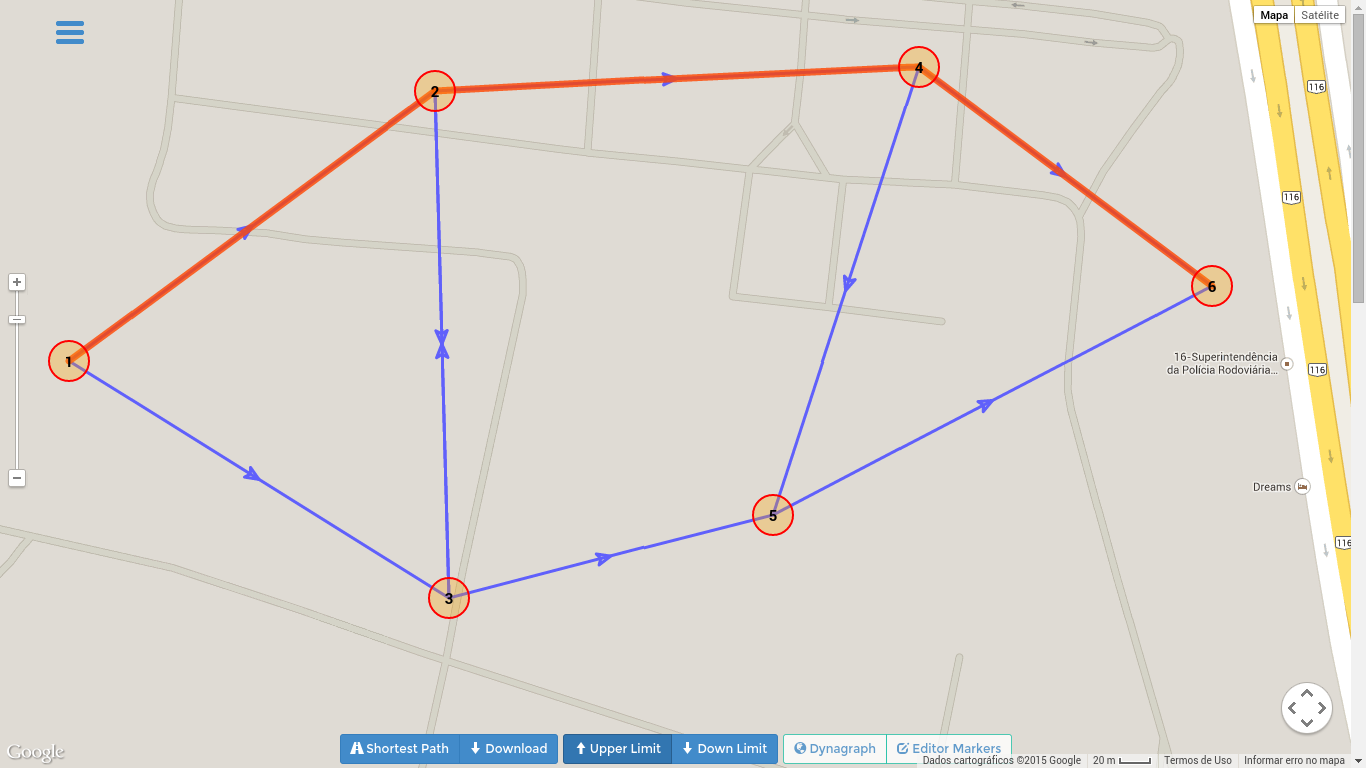
\includegraphics[width=.90\textwidth]{chapters/fig/upperlimit.png}
\caption{Simulador de Caminho Mínimo - Topologia Estática e Atributos Dinâmicos}
\label{fig:upperlimit}
\end{figure}
\FloatBarrier

\begin{figure}[htbp]
\centering
 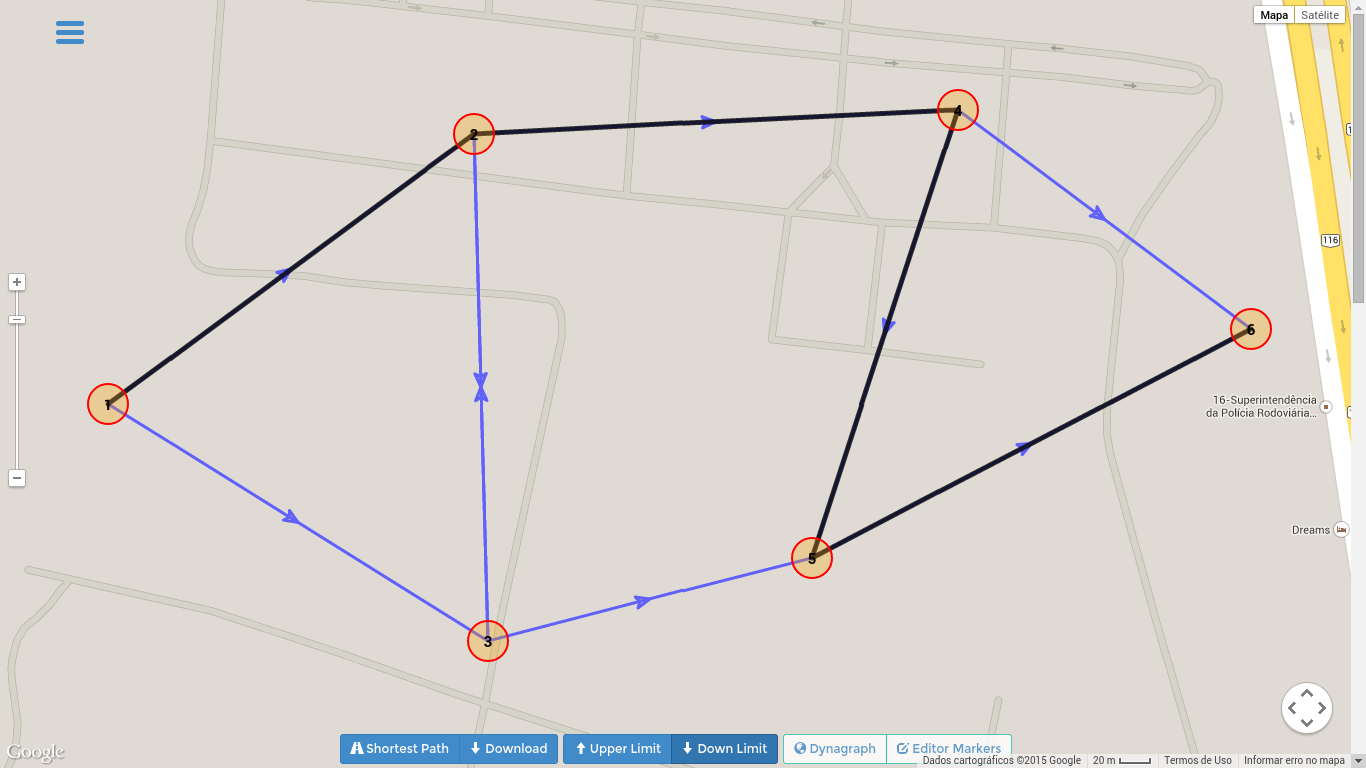
\includegraphics[width=.90\textwidth]{chapters/fig/downlimit.png}
\caption{Simulador de Caminho Mínimo - Topologia Estática e Atributos Dinâmicos: mesma abordagem em \cite{leonard}}
\label{fig:downlimit}
\end{figure}
\FloatBarrier

\begin{center}
  \line(1,0){450}
\end{center}
\lstinputlisting[language=Java]{chapters/dataex1.json}
\begin{figure}[htbp]
  \begin{center}
    \line(1,0){450}
  \end{center}
  \centering
  \caption{Estrutura JSON - Exemplo 1}
  \label{fig:jsondyn}
\end{figure}
\FloatBarrier

A seguir, são apresentados os grafos gerados pela ferramenta de simulação com seus respectivos dados.
